% !TEX root = ../../main.tex
\section{Lắp ráp hoàn thiện sản phẩm}
\label{sec:design-final-assembly}

\begin{figure}[H]
	\centering
	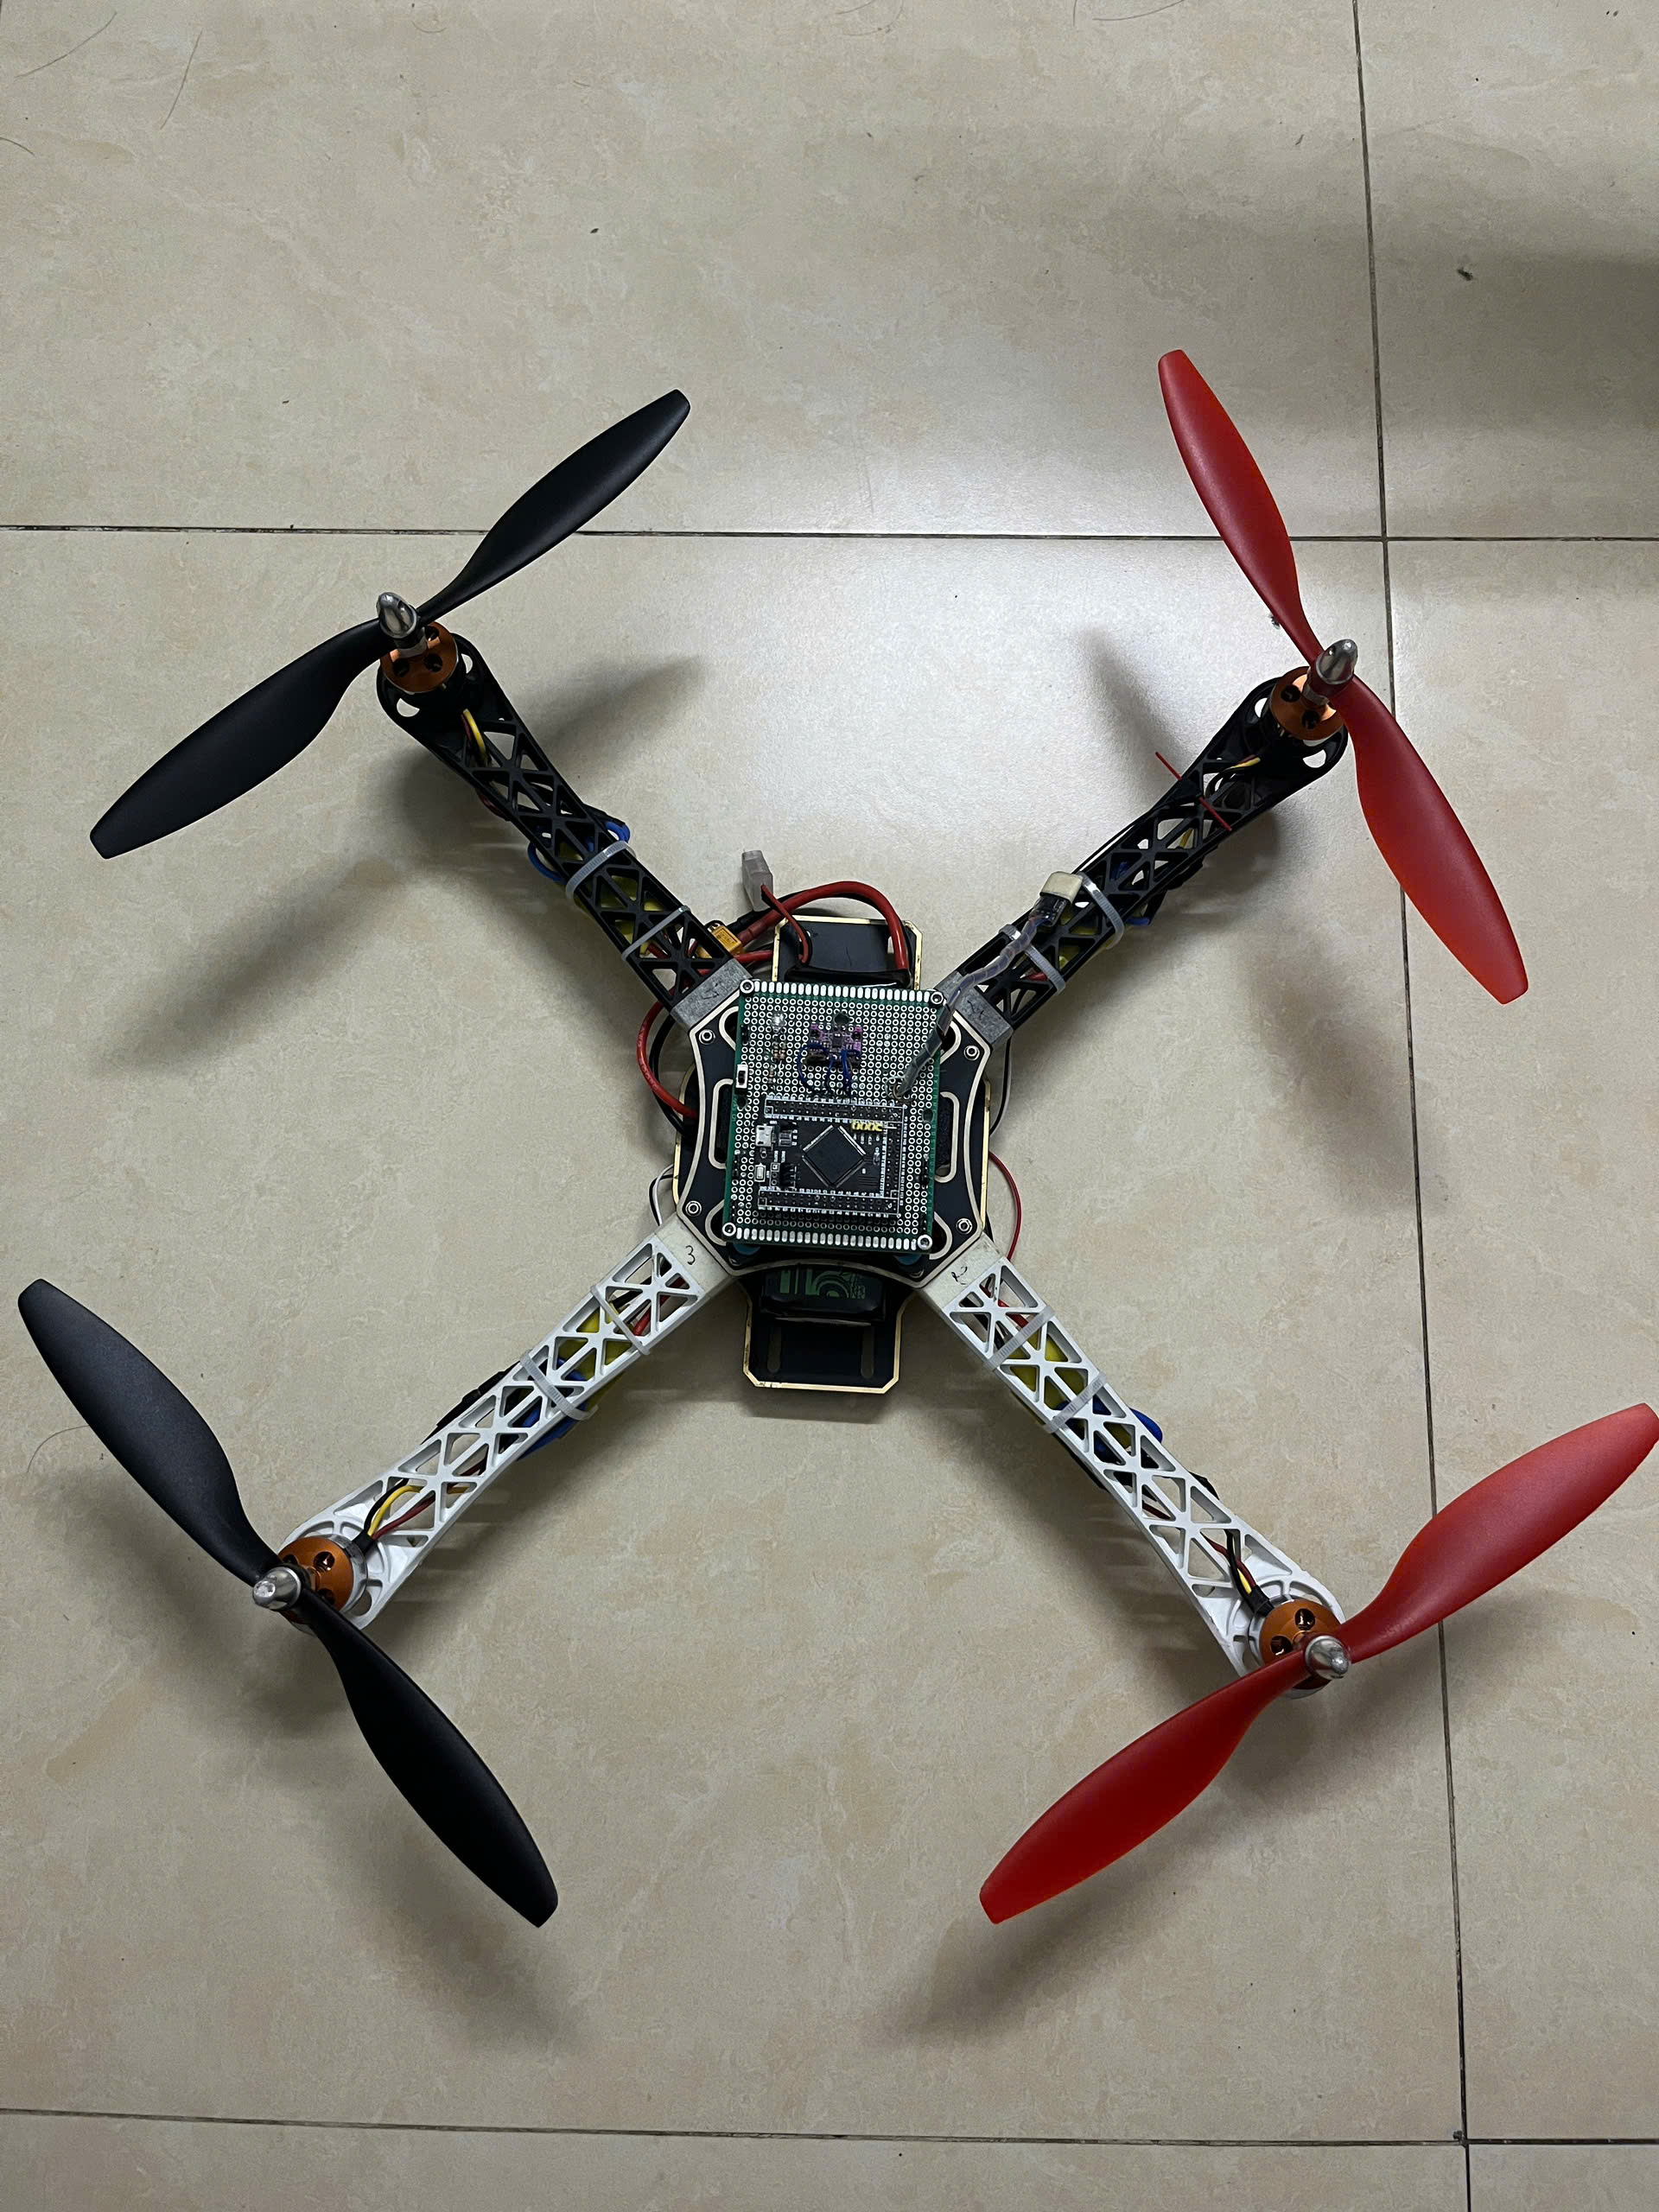
\includegraphics[trim=0 112bp 0 188bp,clip,width=0.95\linewidth,height=13cm,keepaspectratio]{figures/ch03/assembled-quadrotor.jpg}
	\caption{Quadrotor sau khi tích hợp cụm cơ khí, nguồn và điều khiển.}
	\label{fig:design-assembled-quadrotor}
\end{figure}

Cụm điều khiển được gắn trên tấm gá trung tâm, phía trên vị trí pin. Bốn cụm động cơ--cánh quạt phân bố quanh thân theo cấu hình chữ X. Dây nối các cụm được giữ dọc theo tay đòn và đưa về vùng giữa thân; bộ thu vô tuyến cùng anten được bố trí trên một tay đòn, nối với bo điều khiển bằng dây dẫn.

Sau khi tích hợp, hệ động lực, nguồn điện và cụm điều khiển cùng nằm trên một kết cấu khung. Bo xử lý ở phía trên thuận tiện cho việc tiếp cận các chân kết nối, còn pin và đường cấp nguồn tập trung ở thân giữa. Cấu hình lắp ráp này tạo thành mô hình quadrotor phục vụ triển khai chương trình trên STM32 và thử nghiệm điều khiển cân bằng.
